% samplepaper.tex: springer.com
% modificato da MM 06/05/2018
%
\documentclass[runningheads]{llncs}
\usepackage[italian]{babel}
\usepackage{graphicx}
\usepackage{subfigure}
\usepackage{listings}
\usepackage{threeparttable}
% Used for displaying a sample figure. If possible, figure files
% should be included in EPS format.  If you use the hyperref package,
% please uncomment the following line to display URLs in blue roman
% font according to Springer's eBook style:
% \renewcommand\UrlFont{\color{blue}\rmfamily}
\begin{document}
%
\title{Da mettere alla fine degli esperimenti}
%
% \titlerunning{Abbreviated paper title}
% If the paper title is too long for the running head, you can set
% an abbreviated paper title here
%
\author{%
  Alessandro Stefani\inst{1} \and
  Caterina Buranelli\inst{2} \and
  Cristi Gutu\inst{3}}
%
\authorrunning{Alessandro Stefani, Caterina Buranelli, Cristi Gutu}
% First names are abbreviated in the running head.  If there are more
% than two authors, 'et al.' is used.
%
\institute{Corso di laurea in Statistica per le tecnologie e le scienze,
  matricola 1148387 \email{alessandro.stefani.6@studenti.unipd.it} \and Corso di laurea in Statistica per le tecnologie e le scienze,
    matricola 1234567 \email{caterina.buranelli@studenti.unipd.it} \and Corso di laurea in Statistica per le tecnologie e le scienze,
      matricola 1147351 \email{gheorghecristi.gutu@studenti.unipd.it}
  }
%
\maketitle
% typeset the header of the contribution
%
\begin{abstract}
DA FINIRE QUANDO ABBIAMO MESSO A POSTO LA SEZIONE ESPERIMENTI.
Questo progetto tratta la realizzazione attraverso il pacchetto \emph{Whoosh}, di un motore di ricerca
volto al reperimento di documenti della collezione sperimentale \emph{OHSUMED} indicizzata opportunamente.
Il progetto è anche corredato di un webserver che permette all'utente di interrogare il motore di ricerca
in forma interattiva attraverso un browser a scelta.
 \keywords{{\it
      Information Retrieval  \and IR \and statistica \and reperimento \and indicizzazione \and Whoosh \and Python \and webserver \and web \and interrogazione web}}
\end{abstract}

\section{Introduzione}
\label{sec:introduzione}

Lo scopo finale di un Sistema di Information Retrieval (IRS) e' quello di reperire documenti rilevanti relativi a una certa esigenza informativa\footnote{insieme delle circostanze in cui unapersona ha un problema da risolvere o un compito da svolgeree richiede informazioni importanti, utili o necessarie per larisoluzione del problema o lo svolgimento del compito}; dunque i documenti sono il primo ingresso del sistema, mentre il secondo e' costitutito dalle interrogazioni; i documenti devono essere indicizzati e nell'indice creato, si andra' a effettuare la ricerca per reperire documenti rilevanti\footnote{la rilevanza e' la proprieta' che rende l'informazione importante, utile o necessaria a soddisfare l'esigenza informativa dell'utente}. Questa seconda parte e' detta reperimento e non si occupa solo di ricercare tra i documenti, ma anche di riordinare secondo un certo ordine di rilevanza. Cio' che descrive i documenti e cio' che descrive le interrogazioni deve essere confrontabile, infatti nei programmi di indicizzaizone e di reperimento si usa uno schema, che deve essere uguale in entrtambi i casi.
L'indicizzazione e' un trade-off tra il  miglioramento della rapprerentazione del contenuto informativo dei documenti (efficacia) e la gestione degli indici (efficienza). Benche' ci sia sempre tensione tra queste due caratteristiche, ad oggi la questione piu' studiata e' quella dell'efficienza.

Esistono diversi modi per risolvere questo problema, nel nostro caso abbiamo ricercato la configurazione migliore tra un sistema di
reperimento con o senza uso di stopword e il tuning dei parametri dello schema di pesatura\footnote{funzione che assegna per ogni documento diversi livelli d’importanza dei termini mediante dei pesi, che possono variare con l’interrogazione} BM25F .




L'obiettivo principale della relazione \`e da una parte la
documentazione del progetto di un servizio di {IR} e dall'altra una
misura del grado in cui si sia riusciti a mettere in pratica i
contenuti della disciplina illustrati durante le lezioni.

A tal scopo la relazione dovr\`a illustrare nelle sezioni successive:
\begin{itemize}
\item i metodi di indicizzazione,
\item i modelli di reperimento,
\item l'interfaccia basata su un \textit{browser} per il {WWW}
\item i risultati della \emph{valutazione} condotta con la collezione
  sperimentale OHSUMED.
\end{itemize}
Il lettore della relazione \`e lo studente medio di un corso di laurea
in statistica al quale la relazione deve dare tutti gli strumenti per
comprendere il contenuto.  Ci si metta nei suoi panni e si scriva
tutto ci\`o e solo ci\`e che serve.  Chiedersi qual \`e il messaggio
che lo studente deve ``portarsi a casa'', esplicitarlo in questo
paragrafo e concentrarsi su quello nel resto della relazione.

L'introduzione della relazione deve servire al lettore a capire se
vale la pena continuare a leggere il resto.  Si possono riassumere i
contenuti delle sezioni successive e metterne in evidenza i punti
principali.  La relazione consiste di tre paragrafi principali dopo
questa introduzione e prima della bibliografia, per la quale si
suggerisce Bib\TeX\ se si scrive con \LaTeX.

\section{Base di partenza}
\label{sec:base-di-partenza}

La base di partenza \`e formata dai metodi documentati nei libri di
testo.  Si eviti di trascrivere pari pari, si cerchi piuttosto di
rielaborare i contenuti in modo da renderli \emph{coerenti} col resto
della relazione; in particolare, si descrivano tutti e solo i metodi
usati negli esperimenti e si eviti di parlare di quei metodi che poi
non sono stati usati; ad esempio, se si conducono degli esperimenti
con BM25F, si deve descrivere questo schema di pesatura in questa
sezione.
%
%\section{Metodi proposti}
%\label{sec:metodi-utilizzati}
%
%Nel caso in cui si siano sviluppati:
%\begin{itemize}
%\item modelli di reperimento,
%\item metodi di indicizzazione,
%\item schemi di pesatura o
%\item altri metodi o tecniche
%\end{itemize}
%propri, non documentati in libri di testo o altra letteratura, si
%scriva in questa sezione una descrizione accurata e completa.  Si
%mettano in evidenza le caratteristiche distintive dei propri
%contributi.  Se non si \`e proposto nulla di nuovo, si scriva
%\emph{Nessuno}.  In una delle ultime lezioni si vedr\`a come
%implementare delle proprie funzioni di reperimento e schemi di
%pesatura.

\section{Esperimenti}
\label{sec:esperimenti}


Per gli esperimenti si \`e utilizzata parte della gi\`a citata collezione sperimentale chiamata OHSUMED\footnote{ \url{https://bit.ly/2wpOynZ}}.

Si tratta di una collezione di oltre 300'000 articoli provenienti dal database bibliografico MEDLINE pubblicati tra il 1987 ed il 1991, di questi documenti ne sono stati utilizzati 54'711.

I programmi utilizzati per effettuare indicizzazione e reperimento sono stati scritti in python(versione 2.7), in particolare sfruttando oggetti e funzioni del modulo whoosh\footnote{ \url{https://whoosh.readthedocs.io/en/latest/index.html}}.

Per la valutazione dei risultati ottenuti nei vari esperimenti si \`e invece utilizzato lo strumento standard trec\_eval\footnote{ \url{https://trec.nist.gov/trec\_eval/}}.
Questo programma permette di ottenere delle misure della qualit\`a dei risultati di un reperimento effettuato su query di cui si conoscono i documenti da considerare rilevanti.

Come misura da usare nel confronto tra risultati di diverse run si \`e scelta la Mean Average Precision(MAP)\cite{WBC_map} , quantit\`a calcolabile sia a livello di singola query che a livello complessivo su un insieme di query.
Inoltre, per verificare se i valori di MAP ottenuti in run diverse si discostano in modo statisticamente significativo gli uni dagli altri si effettuano test di Wilcoxon su coppie di risultati. \par







Prima di poter iniziare gli esperimenti si \`e dimostrato necessario fare delle scelte riguardo i metodi di reperimento.
Queste scelte sono state fatte in seguito ad alcune run preliminari.

Per la funzione di reperimento e ranking come schema di pesatura si \`e deciso di utilizzare il "Best Match 25 Model with Extension to Multiple Weighted Fields"(BM25F), descritto nella sezione precedente, inquanto "state-of-the-art" dal punto di vista dei modelli per information retrieval su documenti strutturati e come operatore logico per raggruppare le parole delle query si \`e deciso di utilizzare l'operatore OR, ovvero si cercano documenti in cui \`e presente almeno una parola della query.

Sempre a seguito delle run preliminari si \`e deciso di utilizzare, tra i campi delle query, il campo "desc" che d\`a risultati migliori, inoltre, si \`e notato che in alcune query sperimentali sono presenti parole scritte in modo errato e che quindi non risultano presenti nell'indice.
Per questo dopo aver verificato, leggendo i documenti rilevanti per quelle query, dove fossero gli errori, si \`e ritenuto opportuno effettuare una correzione al momento del reperimento.
A grandi linee, la correzione viene fatta su parole che non risultano presenti nell'indice, cercando in quest'ultimo delle parole alternative che si discostano di una lettera rispetto alla parola originale; queste parole vengono quindi aggiunte alla query di partenza e si procede con la ricerca.

Un'ultima scelta \`e stata fatta riguardo il numero massimo di documenti reperiti, si \`e optato per 100 inquanto un numero maggiore non porta grandi miglioramenti dal punto di vista del MAP. \par







Affinch\`e Whoosh possa indicizzare una collezione di documenti, necessita la
specificazione di uno schema, che include per ogni possibile campo dei documenti della collezine, il nome del campo ed il tipo del campo. 
Lo schema di base per la collezione qui utilizzata \`e il seguente:
\par

\begin{lstlisting}
schema = Schema(docid      	= ID(stored=True),
		title      	= TEXT(stored=True),
		identifier	= ID(stored=True),
		terms 		= NGRAM(stored=True),
		authors		= NGRAM(stored=True),
		abstract 	= TEXT(stored=True),
		publication	= TEXT(stored=True),
		source 		= TEXT(stored=True))
\end{lstlisting}
\begin{tablenotes}
      \small
      \item \bf Figura: Schema necessario all'indicizzazione dei documenti. "stored=True" indica che il campo viene salvato ed \`e quindi successivamente accessibile.
    \end{tablenotes}
\par


\subsection{Baseline}
La configurazione baseline ideale, \`e stata scelta in base al Mean Average Precision (M.A.P.)\cite{WBC_map} variando il parametro che indica quale schema di 
pesatura usare nel processo di reperimento tra cui TF\_IDF e BM25F .

 Il processo e codice di indicizzazione sono  facilmente comprensibili visionando il file  \emph{indicizzazione\_batch\_baseline.py}. \par
\lstset{
  language=bash,
  basicstyle=\ttfamily
}

Per eseguire l'indicizzazione  baseline \`e sufficiente lanciare il seguente script python con il comando:
\begin{lstlisting}
  indicizzatore_batch_baseline.py \ 
  cartella_indice file_documenti.xml
\end{lstlisting}

Per eseguire il reperimento che poi produce il file con i risultati in formato compatibile con trec\_eval \`e sufficiente lanciare 
lo script python con il comando:

\begin{lstlisting}
  python search_tk.py cartella_indice \
  file_query.xml cartella_risultati nome_file_risultati
\end{lstlisting}


Descrizione: "1 Campo" significa che il reperimento e' stato eseguito soltanto 
valutando il campo title,   "2 Campi" titolo e abstract,  "3 Campi" titolo e abstract e terms.
\begin{table}
\centering
\begin{tabular}{lll}
\textbf{ 1 Campo }           & \textbf{ 2 Campi }           & \textbf{ 3 Campi }            \\
---------------------------------- & ---------------------------------- & ----------------------------------  \\
 num\textit{q all 63 }       &  num\textit{q all 63 }       &  num\textit{q all 63 }        \\
 num\textit{ret all 37454 }  &  num\textit{ret all 57356 }  &  num\textit{ret all 58456 }   \\
 num\textit{rel all 670 }    &  num\textit{rel all 670 }    &  num\textit{rel all 670 }     \\
 num\textit{rel}ret all 307  &  num\textit{rel}ret all 387  &  num\textit{rel}ret all 383   \\
map all 0.1073               & map all \bf 0.1289               & map all 0.1227               
\end{tabular} 
\begin{tablenotes}
      \small
      \item \bf Figura: Risultati treceval, nessuna manipolazione del testo, numero risultati restituiti per 
ogni query = 1000, pesatura BM25F.
    \end{tablenotes}
\end{table}

Alla luce dei risultati si e' scelto come valori per i parametri baseline: \textit{Documenti rilevanti reperiti}:  387;
\textit{M.A.P}:  0.1289.

\subsection{Primo tentativo: uso delle stopword}

Le stopword\cite{WBC_stopword} sono parole che non portano informazione 
significativa al contenuto informativo come congiunzioni, articoli, avverbi..\par

Inizialmente si \`e pensato di utilizzare le stopword generali della lingua inglese per eliminare le
parole che non portano informazione significativa. I risultati sono stati accettabili, ma siamo riusciti a migliorarli togliendo anche stopword cliniche, cio\`e  strettamente inerenti al contesto medico e abbiamo ottenuto i seguenti risultati:
\begin{table}
\centering
\begin{tabular}{lll}
\textbf{ 1 Campo }           & \textbf{ 2 Campi }           & \textbf{ 3 Campi }            \\
---------------------------------- & ---------------------------------- & ----------------------------------  \\
 num\textit{q all 63 }       &  num\textit{q all 63 }       &  num\textit{q all 63 }        \\
 num\textit{ret all 54873 }  &  num\textit{ret all 612669 }  &  num\textit{ret all 61908 }   \\
 num\textit{rel all 670 }    &  num\textit{rel all 670 }    &  num\textit{rel all 670 }     \\
 num\textit{rel}ret all 477  &  num\textit{rel}ret all 570  &  num\textit{rel}ret all 538   \\
map all 0.2045               & map all \bf 0.2752               & map all 0.1665               
\end{tabular} 
\begin{tablenotes}
      \small
      \item \bf Figura: Risultati treceval, rimozione delle stopword cliniche, numero risultati restituiti per 
ogni query = 1000, pesatura BM25F.
    \end{tablenotes}
\end{table}



%
%Inizialmente si \`e pensato che utilizzare le stopword generali della lingua inglese fosse sufficiente per eliminare le 
%parole che non portano informazione, e di conseguenza aumentare il parametro di interesse M.A.P; i risultati
%non sono stati molto soddisfacenti, abbiamo quindi optato per l'utilizzo di stopword cliniche, cio\`e stopword utilizzate 
%soltato in ambito clinico/medico \cite{stopword_cliniche}.

\begin{thebibliography}{8}

\bibitem{WBC}
W. Bruce Croft and Donald Metzler and Trevor Strohman. Search Engines: Information Retrieval in Practice. Addison Wesley, (2009), pp. 250-252

\bibitem{WBC_stopword}
W. Bruce Croft and Donald Metzler and Trevor Strohman. Search Engines: Information Retrieval in Practice. Addison Wesley, (2009), pp. 90

\bibitem{WBC_map}
W. Bruce Croft and Donald Metzler and Trevor Strohman. Search Engines: Information Retrieval in Practice. Addison Wesley, (2009), pp. 313

\bibitem{stopword_cliniche}
Discovering Related Clinical Concepts Using Large Amounts of Clinical Notes. Ganesan, Kavita and Lloyd, Shane and Sarkar,
 Vikren, (2016), pp. 27-33

\end{thebibliography}

\begin{figure}[h!]
  \subfigure[Alessandro Stefani]{
    
\includegraphics[width=30mm,height=30mm]{aleste}}
  \subfigure[Caterina Buranelli]{
    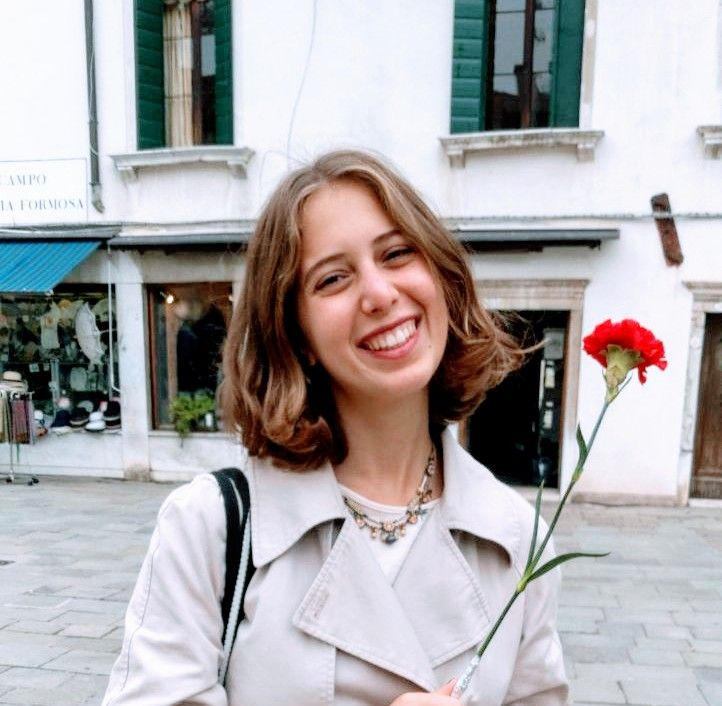
\includegraphics[width=30mm,height=30mm]{caterina}}
  \subfigure[Cristi Gutu]{
    
\includegraphics[width=30mm,height=30mm]{cristi}}
\end{figure}

\end{document}
